\section{Evaluation}\label{sec:evaluation}

We evaluated \xxx on \nreproducedProgs widely used C/C++ programs, including 
three server applications (\apache~\cite{apache} web server, 
\mysql~\cite{mysql} database server, and SSDB~\cite{SSDB} 
key-value store server), one library (\libsafe~\cite{libsafe}), the 4.11.9 Linux 
kernel, and one web browser (\chrome). We used the programs' common performance 
benchmarks as workloads. Our evaluation was done on XXX. 


We focused our evaluation on four key questions:
\begin{tightenum}
	
		
	\item Can \xxx detect known concurrency attacks in the real-world
	(\S\ref{sec:known-attacks})?
	
	\item Can \xxx detect previously unknown concurrency attacks in the real-world
	(\S\ref{sec:unknown-attacks})?
	\item How many false-positive reports from concurrency error 
	detection tools can \xxx reduce (\S\ref{sec:reduce})?
	
	\item How many potential victim inputs can \xxx indicate(\S\ref{sec:overview})?
		
	
\end{tightenum}

\subsection{Detecting Known and New Concurrency Attacks}


We applied \xxx on \nknownVul concurrency attacks listed in 
Table~\ref{tab:known_attacks}. \xxx detected all the vulnerabilities.
Currently \xxx incorporates two race detectors. There are other
types of concurrency bugs that can also lead to concurrency attacks, including
atomicity violations~\cite{lu:concurrency-bugs}. Atomicity violations 
can be detected by other detectors (\eg, CTrigger~\cite{ctrigger:asplos09}). By 
integrating these detectors (future work), \xxx's analysis and verifier 
components can detect more concurrency attacks.


Because all \xxx's dynamic verifiers of are implemented based on \lldb, which 
only supports applications, we haven't run these verifiers in Linux kernel. 
Nevertheless, \xxx's static vulnerability analyzer was applied to the Linux 
kernel and detected the evaluated concurrency attacks. For Linux kernel, our 
dynamic verifiers can be implemented in QEMU~\cite{qemu}. We leave the 
implementation in future work.

Aside from the discussed known and unknown concurrency attacks, \xxx generates 
180 reports in total. Due to the lack of domain knowledge and semantic 
understanding of program code, we didn't verify all of these 
potential vulnerability reports yet. These reports could either be benign 
races or new concurrency attacks. Nevertheless, by 
greatly reducing the number of reports from 31K to 
180 (Table~\ref{tab:reduce},
\xxx has greatly mitigated developers' burdens.






\begin{table*}[h]
	\footnotesize
	\centering
	\vspace{-.05in}
	\begin{tabular}{lrrrrr}
		{\bf Name} & {\bf Vul. Type} & {\bf Subtle Inputs}  & {\bf Bug Known}  & {\bf Attack Known} \\
		\hline\\[-1.3ex]
		% \multirow{2}{*}{\apache-2.0.48} & Double Free & Y & \cmark \\
		% & Buffer Overflow & N & \cmark \\
		\apache-2.0.48 & Double Free & PhP queries & Yes  & Yes \\
		% \hline
		% \apache-2.2.10     & Integer Overflow & N & \cmark \\
		\hline
		\chrome-6.0.472.58 & Use after free & Js console.profile  & Yes  & Yes \\
		\hline
		\libsafe-2.0-16    & Buffer Overflow  & Loops with \v{strcpy()}  & Yes  & Yes \\
		\hline
		%\libvirt-1.2.0     & Null Ptr Deref  & Y & \xmark \\
		%\hline
		\linux-2.6.10      & Null Func Ptr Deref & Syscall parameters & Yes  & Yes \\
		\hline
		\linux-2.6.29      & Privilege Escalation & Syscall parameters  & Yes  & Yes \\
		\hline
		\mysql-5.0.27      & Access Permission & FLUSH PRIVILEGES & Yes  & Yes \\
		\hline
		\mysql-5.1.35      & Double Free & SET PASSWORD & Yes  & Yes \\
		%\ssdb                   &  12   &  0  & 0   &  0 & 3  \\
		%\chrome           &   X  & X   &  X & X  \\
	    \hline
		\linux-4.11.9(CVE)      & Buffer Overflow & Three Syscalls & No & No \\
        \hline
	    \apache-25520      & Buffer Overflow & Loop     & Yes  &No  \\
	   
		\hline\\[-2.3ex]                                          
	\end{tabular}
	\vspace{-.05in}
	\caption{{\em \xxx's detection results on concurrency attacks.} \rm 
		{With the listed subtle inputs, all these attacks were often 
			triggered within 20 repeated queries or loops except the \apache one.}} 
	\label{tab:attacks}
	\vspace{-.1in}
\end{table*}


\xxx detected \nunknownVul previously unknown concurrency attacks caused by 
one new data race and two known data races. Analyzing whether known data races 
can lead to unknown concurrency attacks is still crucial (\S\ref{sec:findings}), 
because once attackers break in, they may remain latent for a long time.

% In this section, we are going to elaborate through these 
% new concurrency attacks in detail. We
% will also discuss why previous tools failed to detect these attacks.

\begin{figure}[h]
	\centering
	% \vspace{-.1in}
	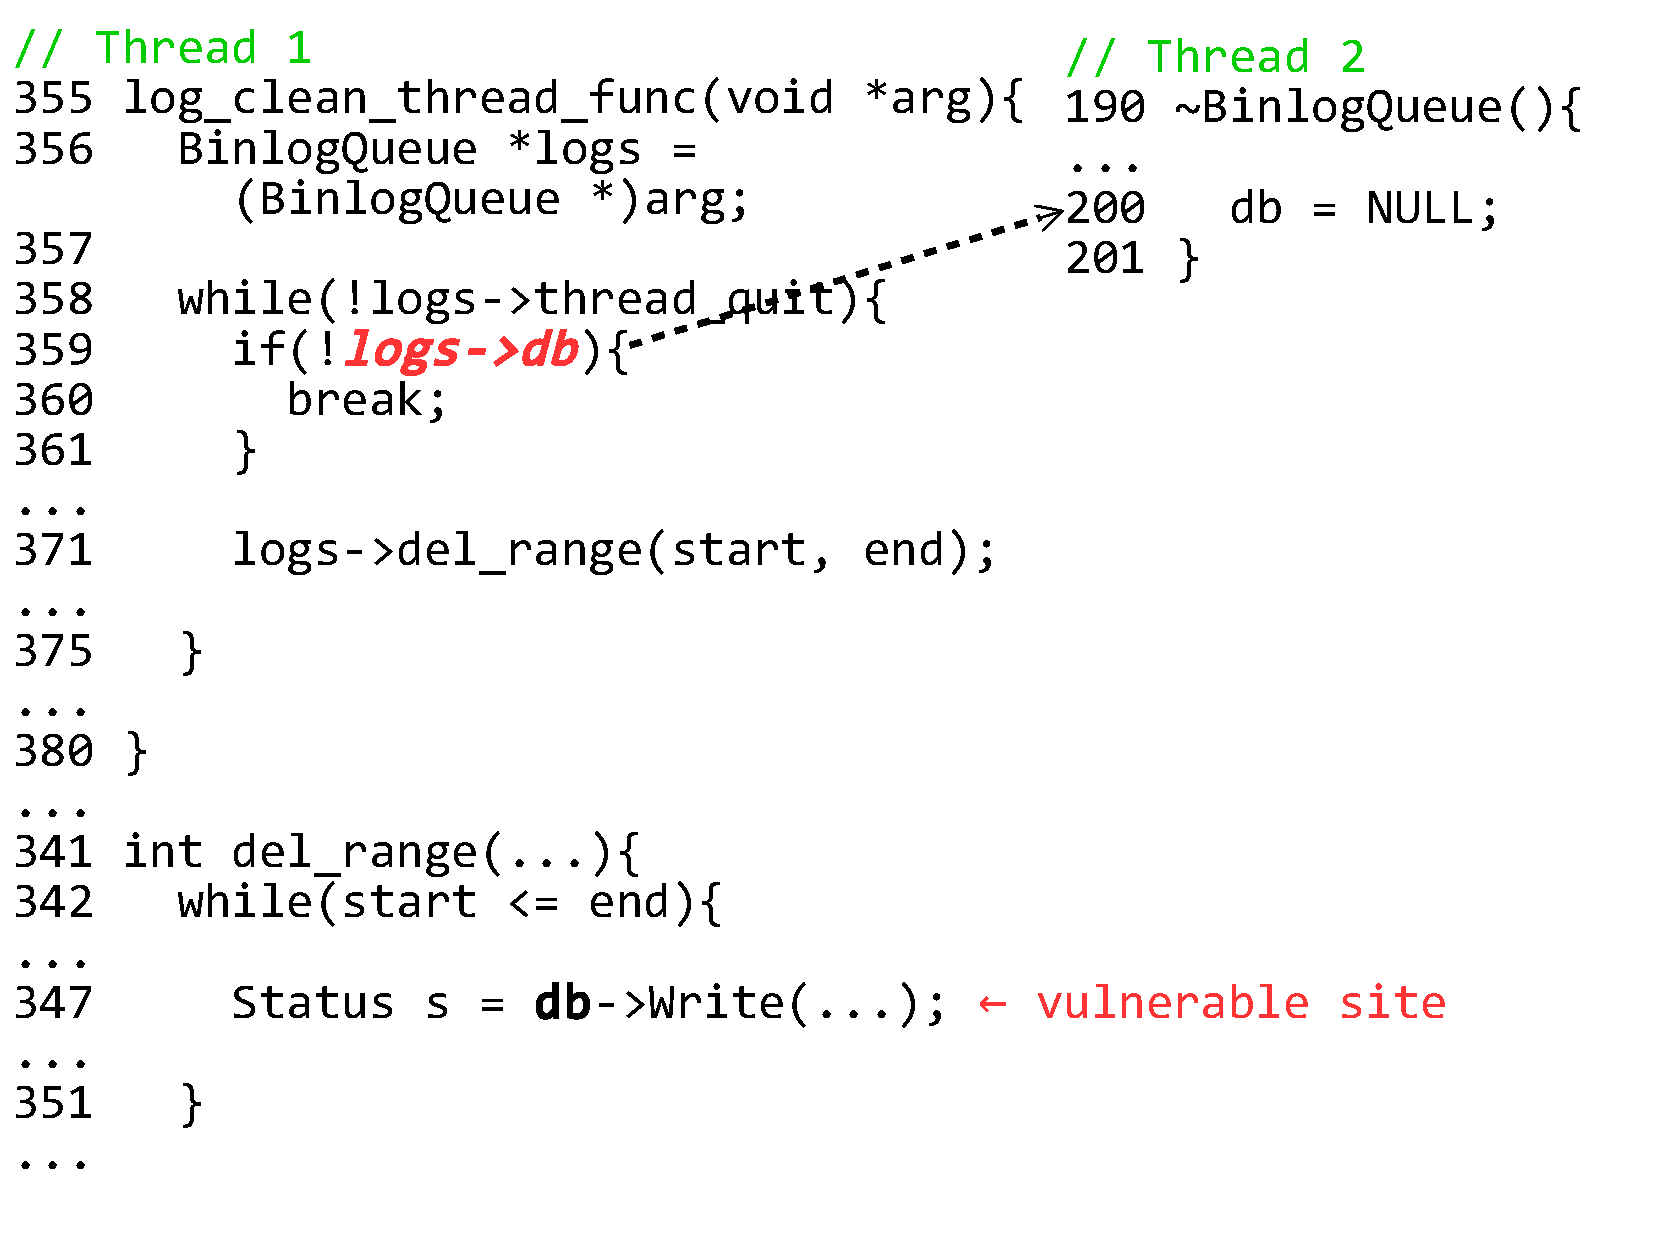
\includegraphics[width=0.9\columnwidth]{figures/ssdb}
	\vspace{-.25in}
	\caption{{\em A new concurrency bug and attack in \ssdb-1.9.2.}} 
	\label{fig:ssdb}
	\vspace{-.2in}
\end{figure}

\xxx detected a new data race and a previously unknown use-after-free 
concurrency attack in \ssdb. Figure~\ref{fig:ssdb} shows the details of 
this vulnerability. During server shutdown, \ssdb uses adhoc synchronization to 
synchronize between threads. However, it's possible that line 359 is executed 
before line 200. This race causes \v{log\_clean\_thread\_fun} to fail to break 
out of the while loop. Moreover, \v{log\_clean\_thread\_fun} could execute 
\v{del\_range} which could use \v{db} and cause a use after free. Even 
more, line 347 is a function pointer dereference which could cause log 
corruption or program crash if the memory area was reused by other threads.

\xxx's static analyzer (\S\ref{sec:algo}) identified the vulnerability site at 
line 347 because it is a pointer dereference. This site is 
control dependent on the corrupted branch on line 359. \xxx's dynamic 
vulnerability verifier (\S\ref{sec:vulnerability_verifier}) further verified 
that the other thread will free the memory area and set the pointer to NULL 
before the dereference within current thread. We reported this race and attack 
to \ssdb developers.

\begin{figure}[h]
	\centering
	\vspace{-.15in}
	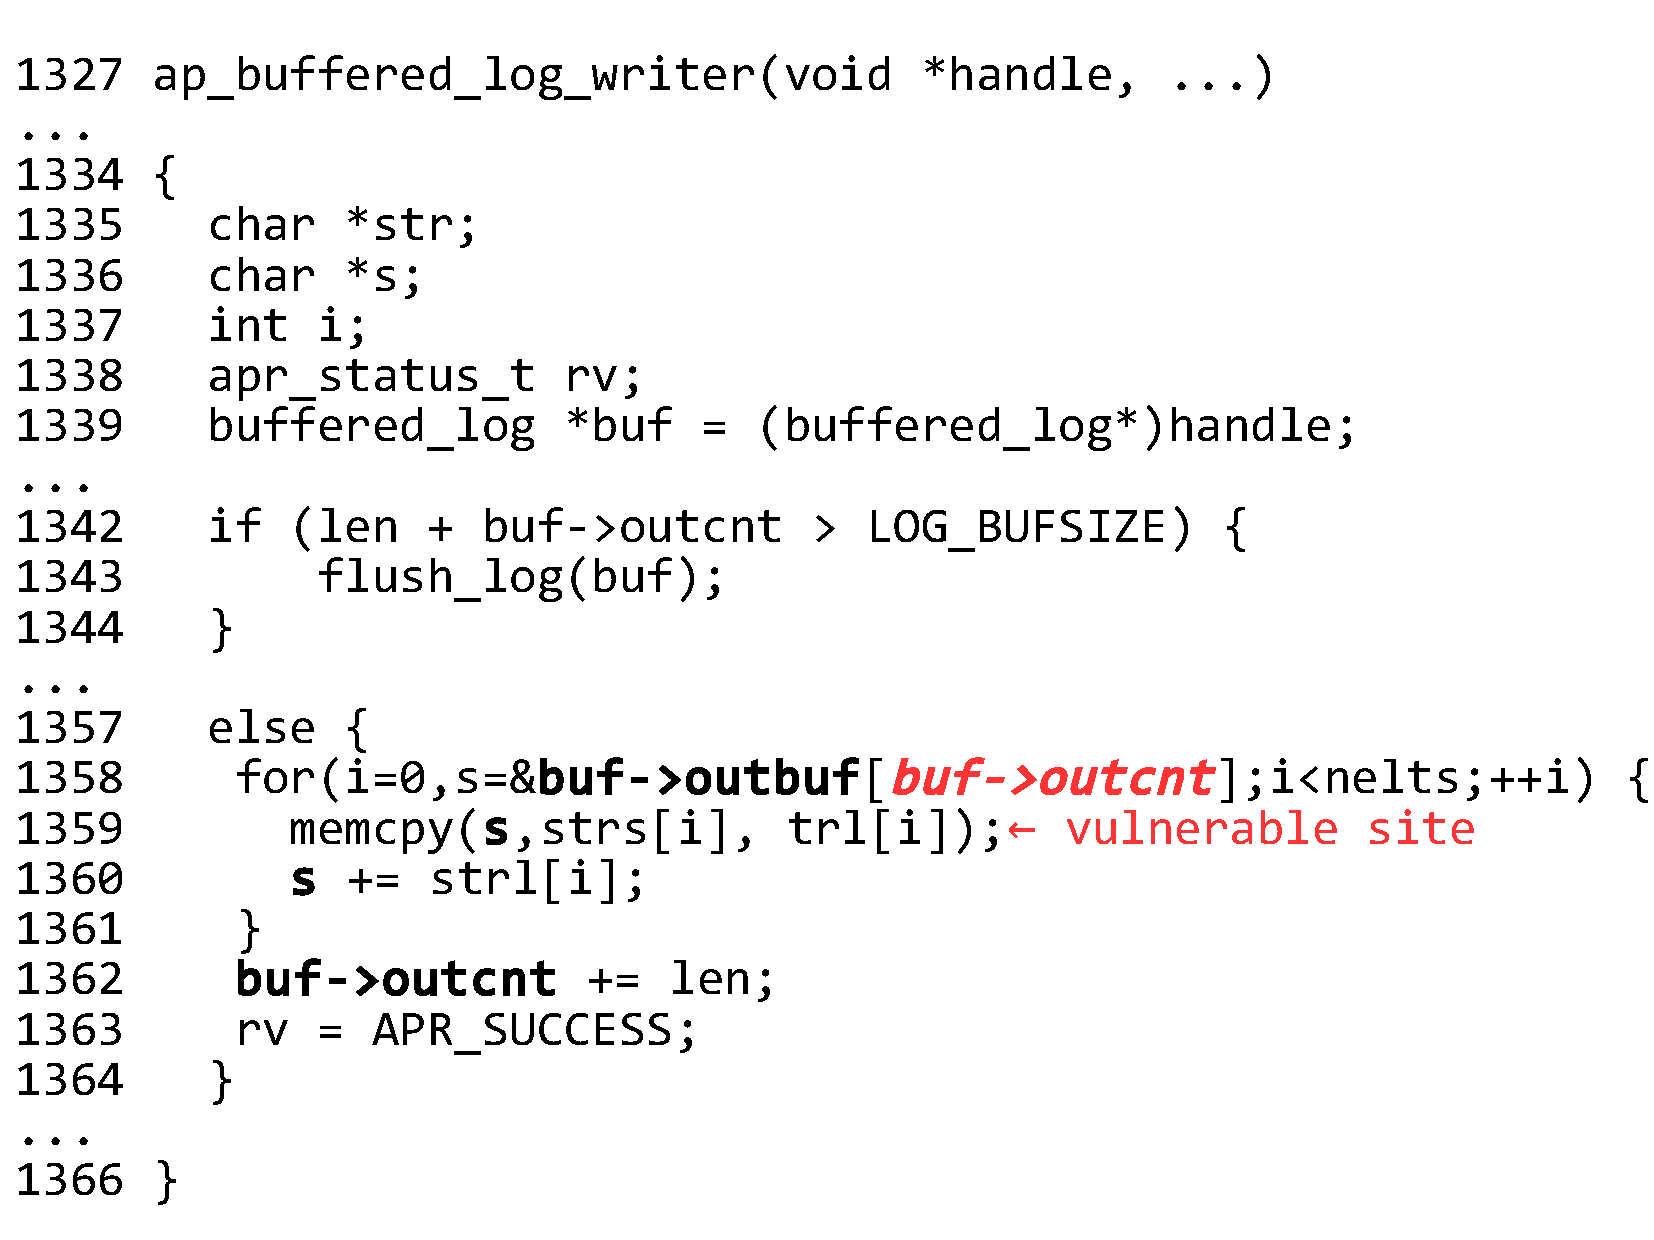
\includegraphics[width=0.9\columnwidth]{figures/apache-25520}
	\vspace{-.15in}
	\caption{{\em A new HTML integrity violation in \apache-2.0.48.}} 
	\label{fig:apache-25520}
	\vspace{-.1in}
\end{figure}

The second previously unknown concurrency attack stems from a known 
data race in \apache. This attack made \apache's own request logs be written 
into other users' HTML files stored in \apache, causing a HTML integrity 
violation and information leak. Figure~\ref{fig:apache-25520} shows the code of 
this vulnerability from the Apache-25520 bug~\cite{apache-bug-25520}.
\v{buf->outcnt} is shared among threads and serves as an index of a buffer
array. Due to a lack of proper synchronization when modifying this variable on
line 1362, a data race occurred and caused the server to write wrong 
contents to \v{buf->outbuf}. 

Worse, the wrong contents could also overflow \v{buf->outbuf} and cause a
buffer overflow. Even worse, \apache stores the file descriptor of its 
HTTP request log next to \v{buf->outbuf}. We constructed a one-byte 
overflow of \v{buf->outbuf}, corrupted this file descriptor, and made 
\apache's own HTTP request logs be written to an HTML file with the 
exact corrupted value of this file descriptor.

Although this data race has been well studied 
by researchers~\cite{lu:concurrency-bugs}, people thought the worst 
consequence of this bug would just be corrupting \apache's own request log. 
We were the first to detect this HTML integrity violation attack with \xxx 
and the first to construct the actual exploit scripts. 
% Leveraging this corruption, we made \apache write its HTTP request 
% logs to a particular html file stored in this server, which causes a severe
% integrity violation attack.

\xxx's vulnerability analysis (\S\ref{sec:algo}) pinpointed the vulnerable site 
at line 1359 and inferred that this line is data dependent on the corrupted 
variable on line 1358. \xxx's dynamic race verifier (\S\ref{sec:verify-race}) 
triggered the race and showed how many bytes in
\v{buf->outbuf} were overflowed.

\begin{figure}[h]
	\centering
	\vspace{-.15in}
	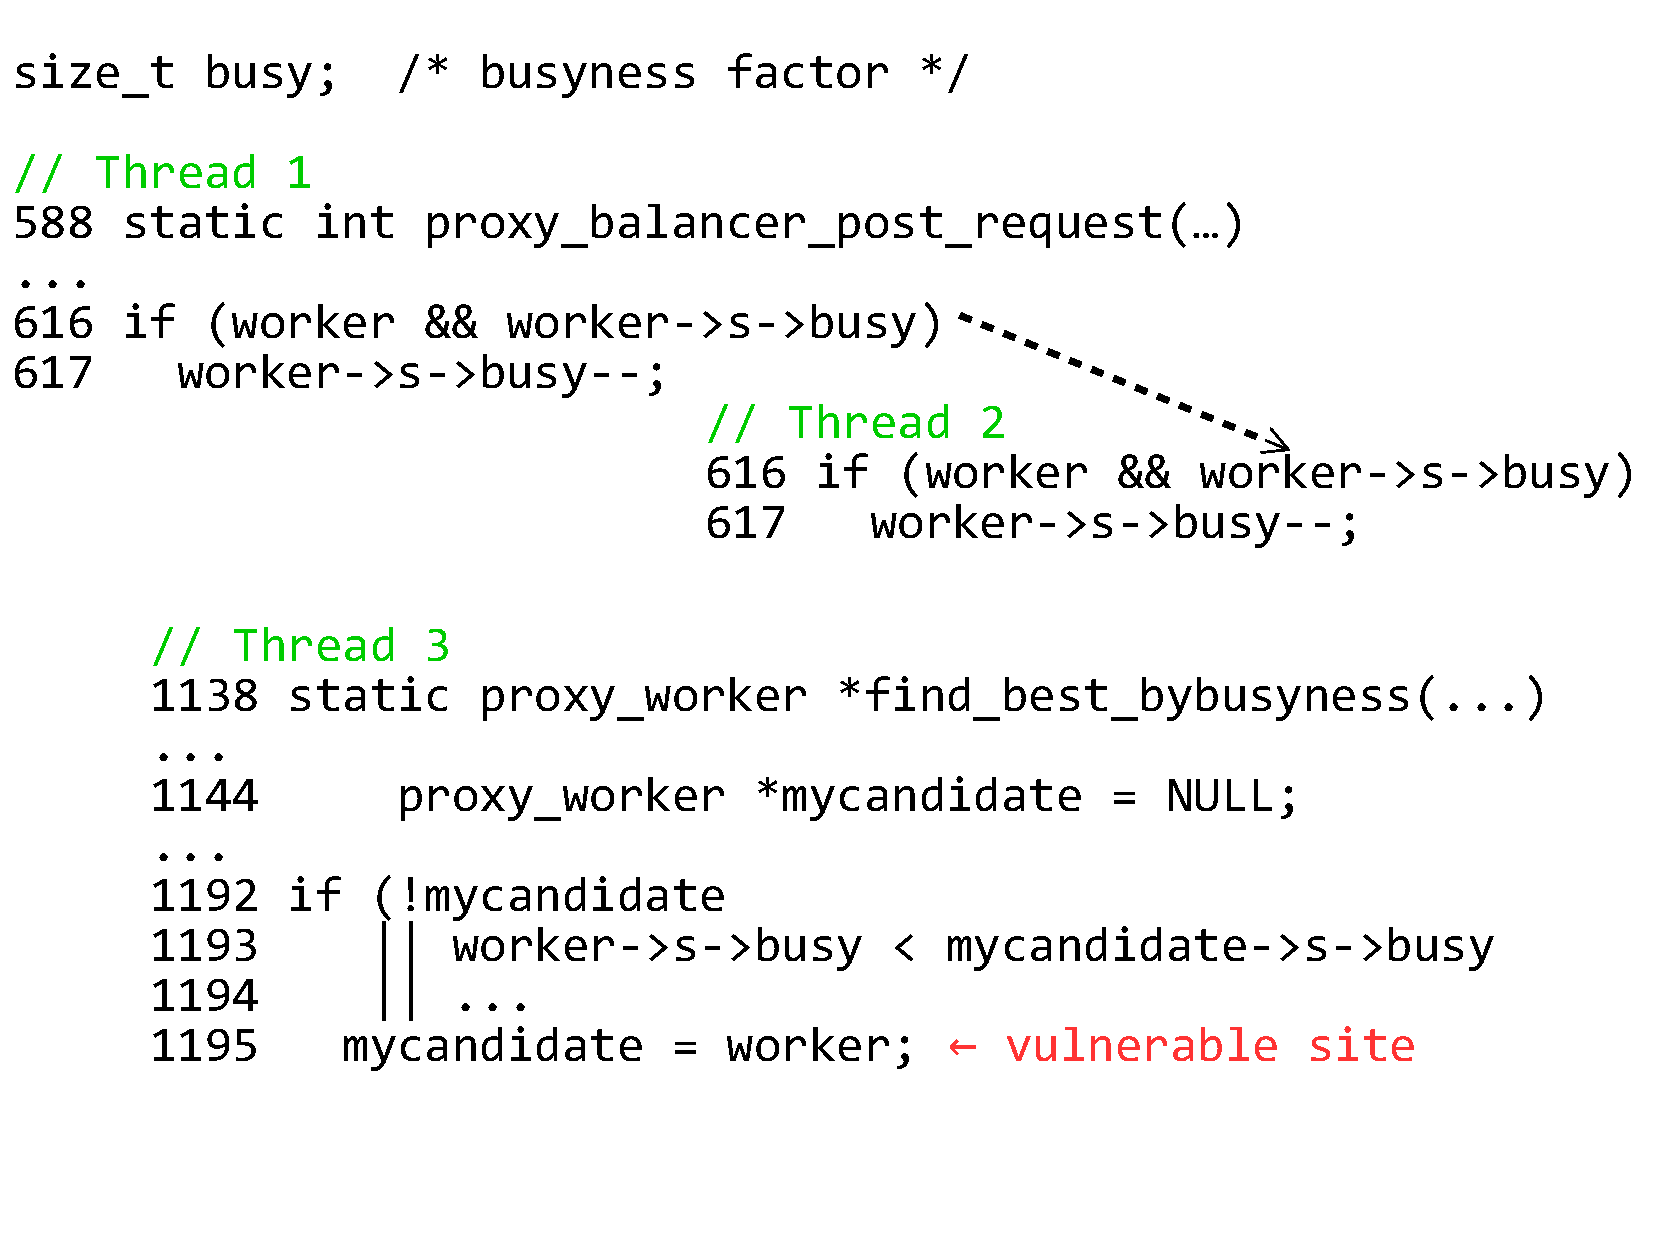
\includegraphics[width=0.85\columnwidth]{figures/apache-46215}
	\vspace{-.4in}
	\caption{{\em A new integer overflow and DoS attack based on \apache-46215.}} 
	\label{fig:apache-46215}
	\vspace{-.1in}
\end{figure}

% Moreover, we've detected an integer overflow vulnerability that could cause a 
% worker thread to be absolutely
% ignored by load balancer for incoming requests based on a previously reported 
% bug. 
% This attack causes degraded server performance or DOS attack in the worst 
% case. 
The third previously unknown concurrency attack was an integer overflow DoS 
attack based on a known \apache-46215 data race. Figure~\ref{fig:apache-46215} 
shows the \apache-46215 bug~\cite{apache-bug-46215}. Each \apache worker thread 
contains a field \v{worker->s->busy} to indicate its busyness. An \apache 
load balancer component contains threads to concurrently increment or decrement 
these flags for worker threads when they start or finish serving requests. 
However, as shown in line 616, this is a data race because developers forgot to 
use a lock during the counter increment and decrement.

Over years, this busyness counter has been viewed a statistic and its 
data race does not matter much. Unfortunately, this counter is an unsigned 
integer, and an integer overflow could be triggered during the decrement and 
could make the counter the largest unsigned integer (\ie, marking a thread the 
``busiest" one). The check in line 617 can be easily bypassed because of the 
race. Because load balancer assigns future requests based on the worker 
threads' counters, arbitrary worker threads in \apache can be viewed the 
busiest ones and be completely ignored, causing a DoS attack on these threads 
and a significant downgrade of \apache's throughput.

\xxx detected this concurrency attack as follows. \xxx's race detector detected 
a race between line 617 and line 1192. \xxx's dynamic race verifier reported 
a detailed dynamic race information including the racing instructions, the 
value they could read or write to the variable and the type of the variable. 
We then found \v{worker->s->busy} in some worker threads had an overflowed 
value: \v{18,446,744,073,709,551,614}. \xxx's vulnerability analysis 
(\S\ref{sec:algo}) reported that a pointer assignment could be control dependent 
on the corrupted branch of line 1192. \xxx's vulnerability verifier verified 
that the branch was indeed corrupted and line 1195 was reachable.
% We also
% found out what requests the workers were executing at that time by manually 
% inspecting program states and used those type of requests as vulnerable 
% inputs. 

These three previously unknown concurrency attacks were overlooked by 
prior reliability and security tools mainly due to three reasons. First, 
compared to \xxx's reduced vulnerable reports, the data races of these three 
attacks were buried within at least 87X more false reports in \apache and 6X 
more in \ssdb produced by the prior \tsan race detector. Second, without 
\xxx's static bug-to-attack propagation analysis (\S\ref{sec:algo}), even though 
the races can be detected by existing race detectors, the security 
consequences of these bugs were unknown to detectors. Third, without 
\xxx's dynamic race verifier (\S\ref{sec:verify-race}) and 
vulnerability verifier (\S\ref{sec:vulnerability_verifier}), whether these 
races and their attacks can be realized were unknown either.



\subsection{Reducing False-positive Race Reports}

Table~\ref{tab:reduce} shows \xxx's race report reduction results. The 
second
column indicates the number of raw reports generated by our race detector.
The third column shows how many adhoc synchronizations we found.
The fourth column shows how many reports
our dynamic race verifier had removed. The fifth column shows the number of the 
remaining reports.

Overall, \xxx is able to prune 94\% cases of false positives in Linux kernel 
and 97.7\%
for the other applications. This significant reduction will help developers save
much diagnostic time. The performance of \xxx's static analysis tool is critical
because \xxx aims to be scalable to large programs. The last column of
Table~\ref{tab:reduce} shows the average time 
cost of \xxx's static analysis tool per bug report. Overall, except for Linux 
kernel and \chrome, \xxx's analysis finished analyzing each program's bug 
reports within a few hours.


\begin{table}[ht!]
	\footnotesize
	\centering
	\begin{tabular}{l|r|r|r|r|r|r|r}
		{\bf Name} & {\bf LoC} & {\bf \# r.r.}& {\bf \# \xxx's r.} & {\bf \# atks} & {\bf \# atks found}  \\
		\hline
		\apache    &    290K    &   715  &  10   &  3  & 3 \\
		\chrome    &   3.4M   & 1715  &  115 &  1  & 1 \\
		\libsafe   &   3.4K     & 3  & 3 & 1 &  1 \\
		\linux     &     2.8M    & 24641  & 34  &  2  & 2  \\
		\mysql     &    1.5M    & 1123 &  16  &  2  & 2 \\
		\ssdb      &  67K   &  12  &  2  &  1  & 1  \\
		\hline\\[-2.3ex]
		Total      &   -    &  -  &  - &  - & - \\
	\end{tabular}
	\vspace{-.1in}
	\caption{{\em \xxx race report reduction and concurrency attack detection results.} \rm {Description}} 
	\label{tab:raduce}
	\vspace{-.2in}
\end{table}

\subsection{Find potential victim inputs}






\begin{table}[ht!]
	\footnotesize
	\centering
	\begin{tabular}{l|r|r|r|r|r|r|r}
		{\bf Name} & {\bf Type} & {\bf \# Fed Inputs}& {\bf \# Victim Inputs} & {\bf \# atks}  \\
		\hline
		\apache    &   apr\_palloc   &  -   &  -  & -  \\
		\linux     &  kmalloc  & 180   &  6  &  1   \\
		\hline\\[-2.3ex]
		Total      &    -     &  -  & -  & -\\
	\end{tabular}
	\vspace{-.1in}
	\caption{{\em \xxx's Concurrency Fuzzer.} \rm {Description}} 
	\label{tab:fuzzer}
	\vspace{-.2in}
\end{table}


